\chapter{Инженерно-геологический разрез}\label{app:razrez}

\begin{figure}[ht]
  \centerfloat{
    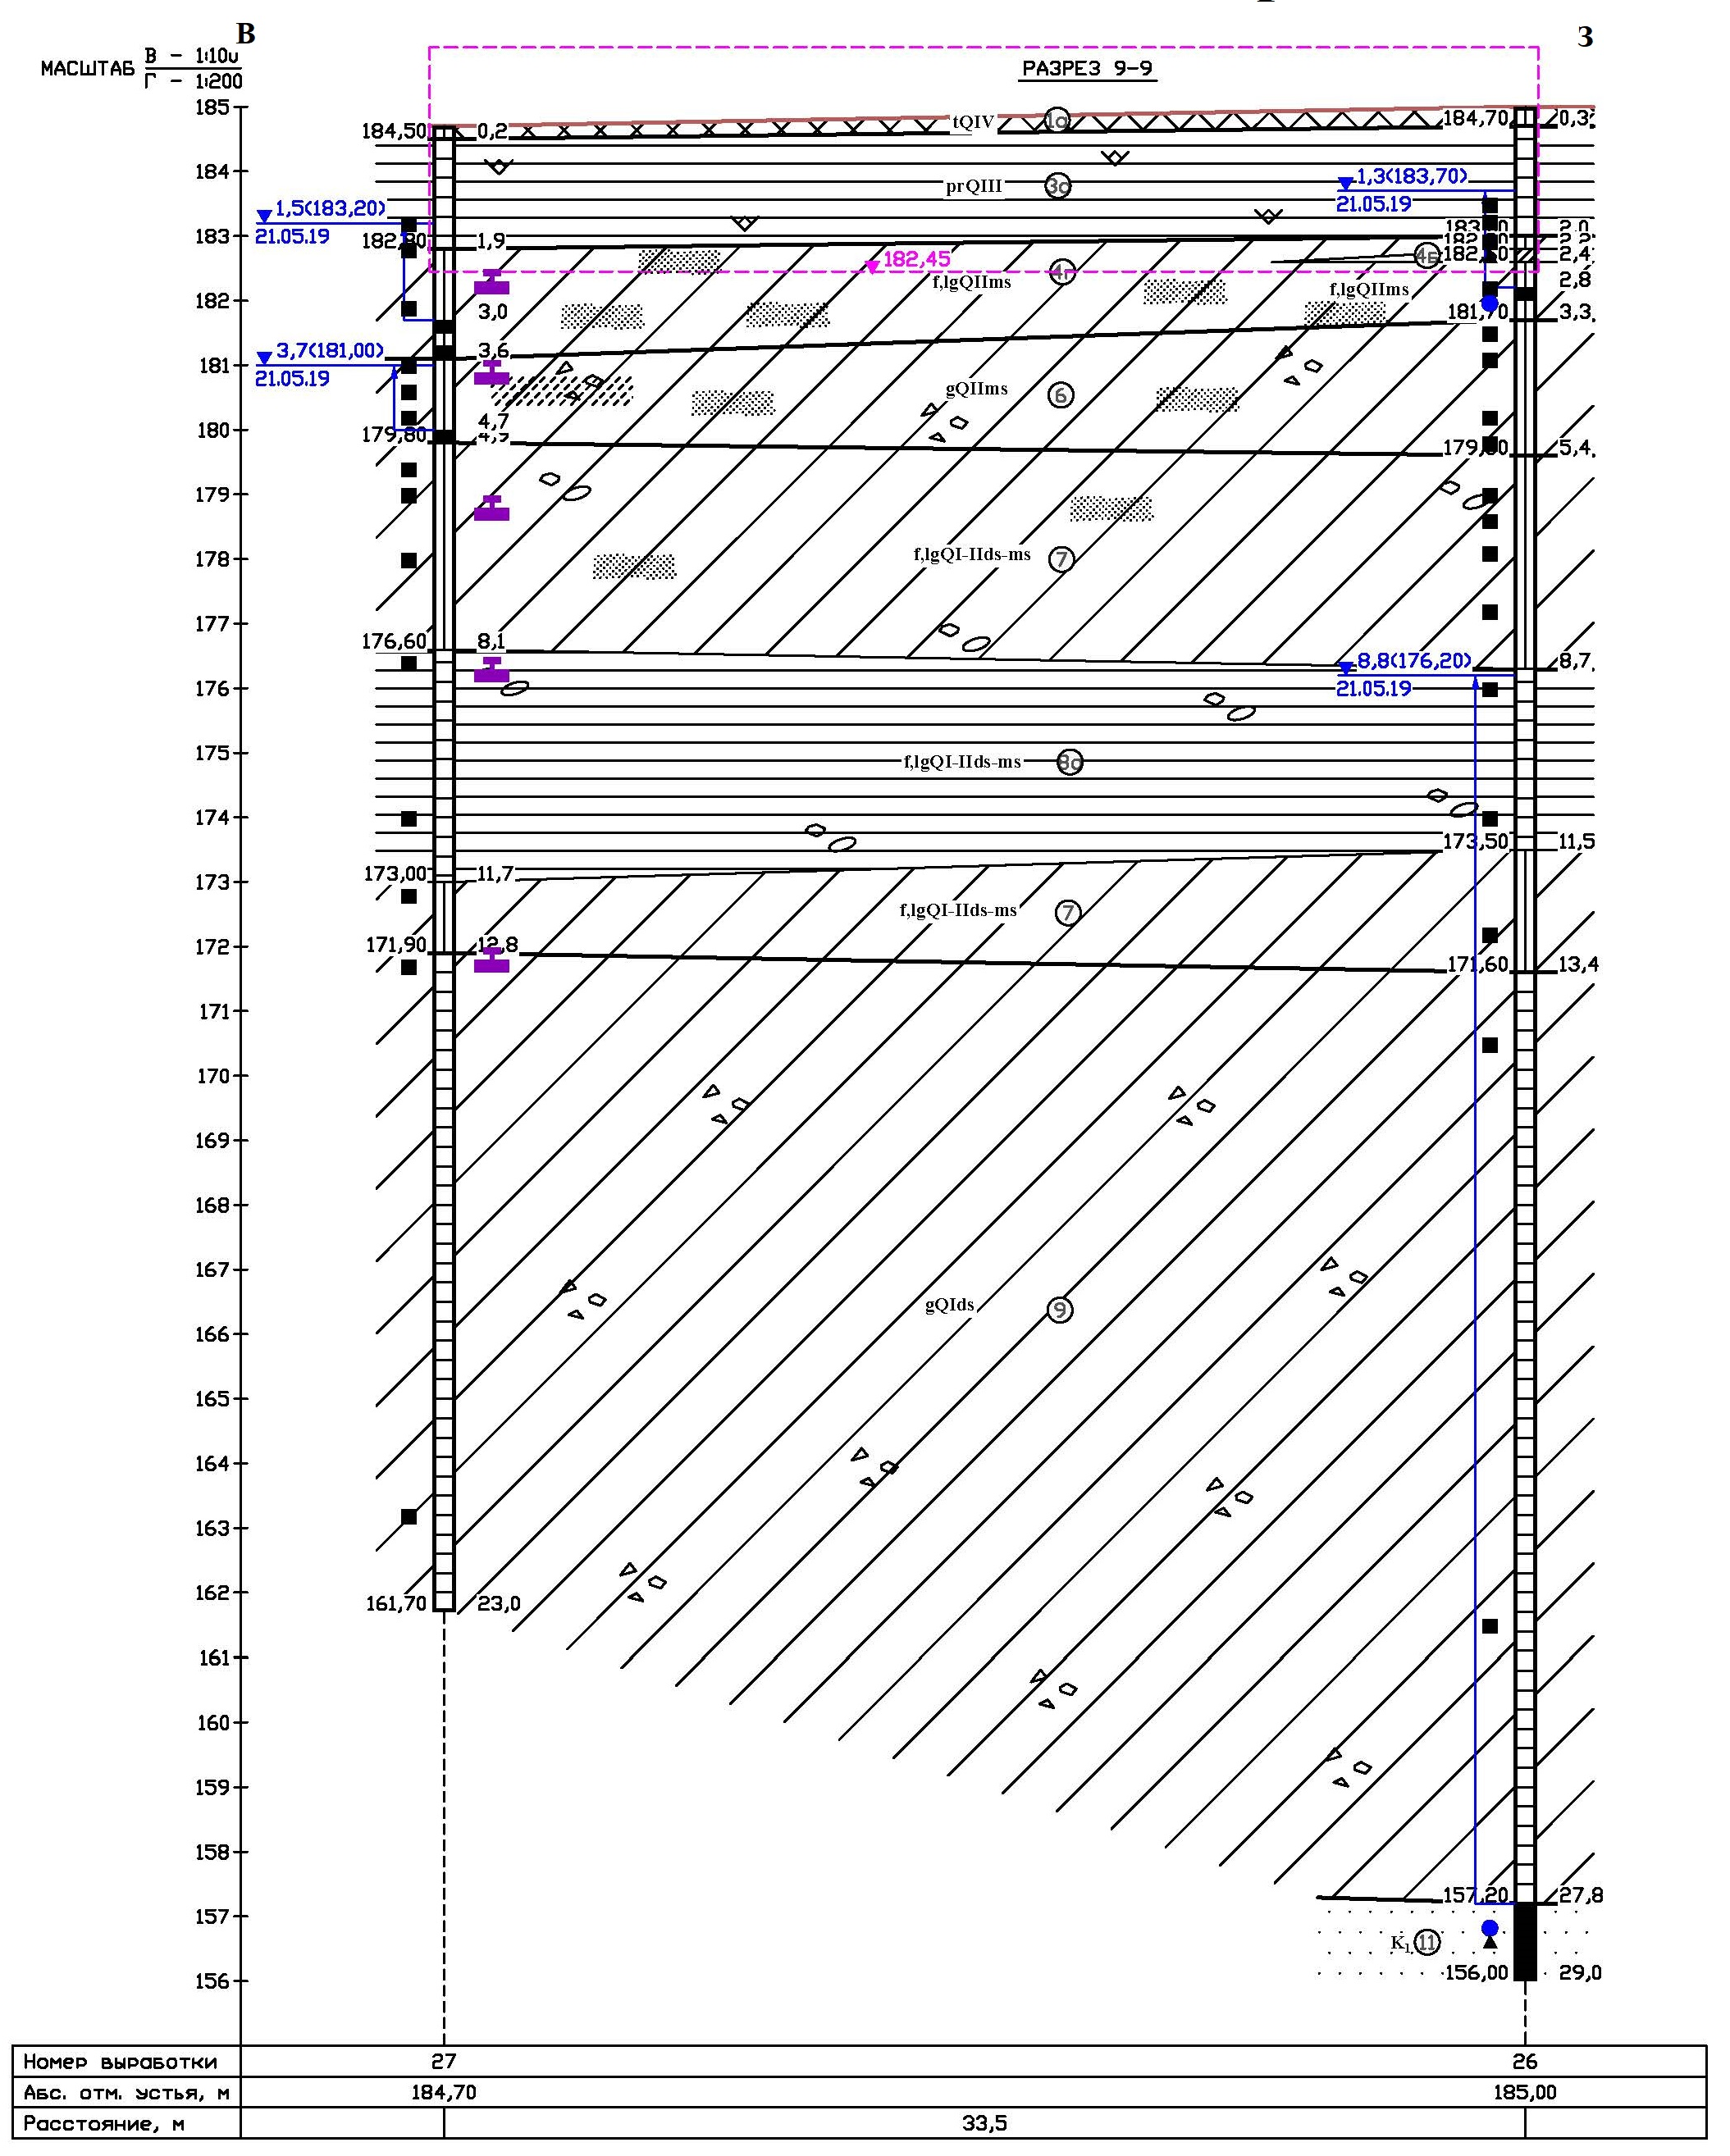
\includegraphics[scale=0.36]{images/razzr.png}
  }
  \caption{Инженерно-геологический разрез исследуемой территории (Технический отчет. Саларьево-парк, 2019)}\label{fig:fig}
\end{figure}

\begin{figure}[ht!]
  \centerfloat{
    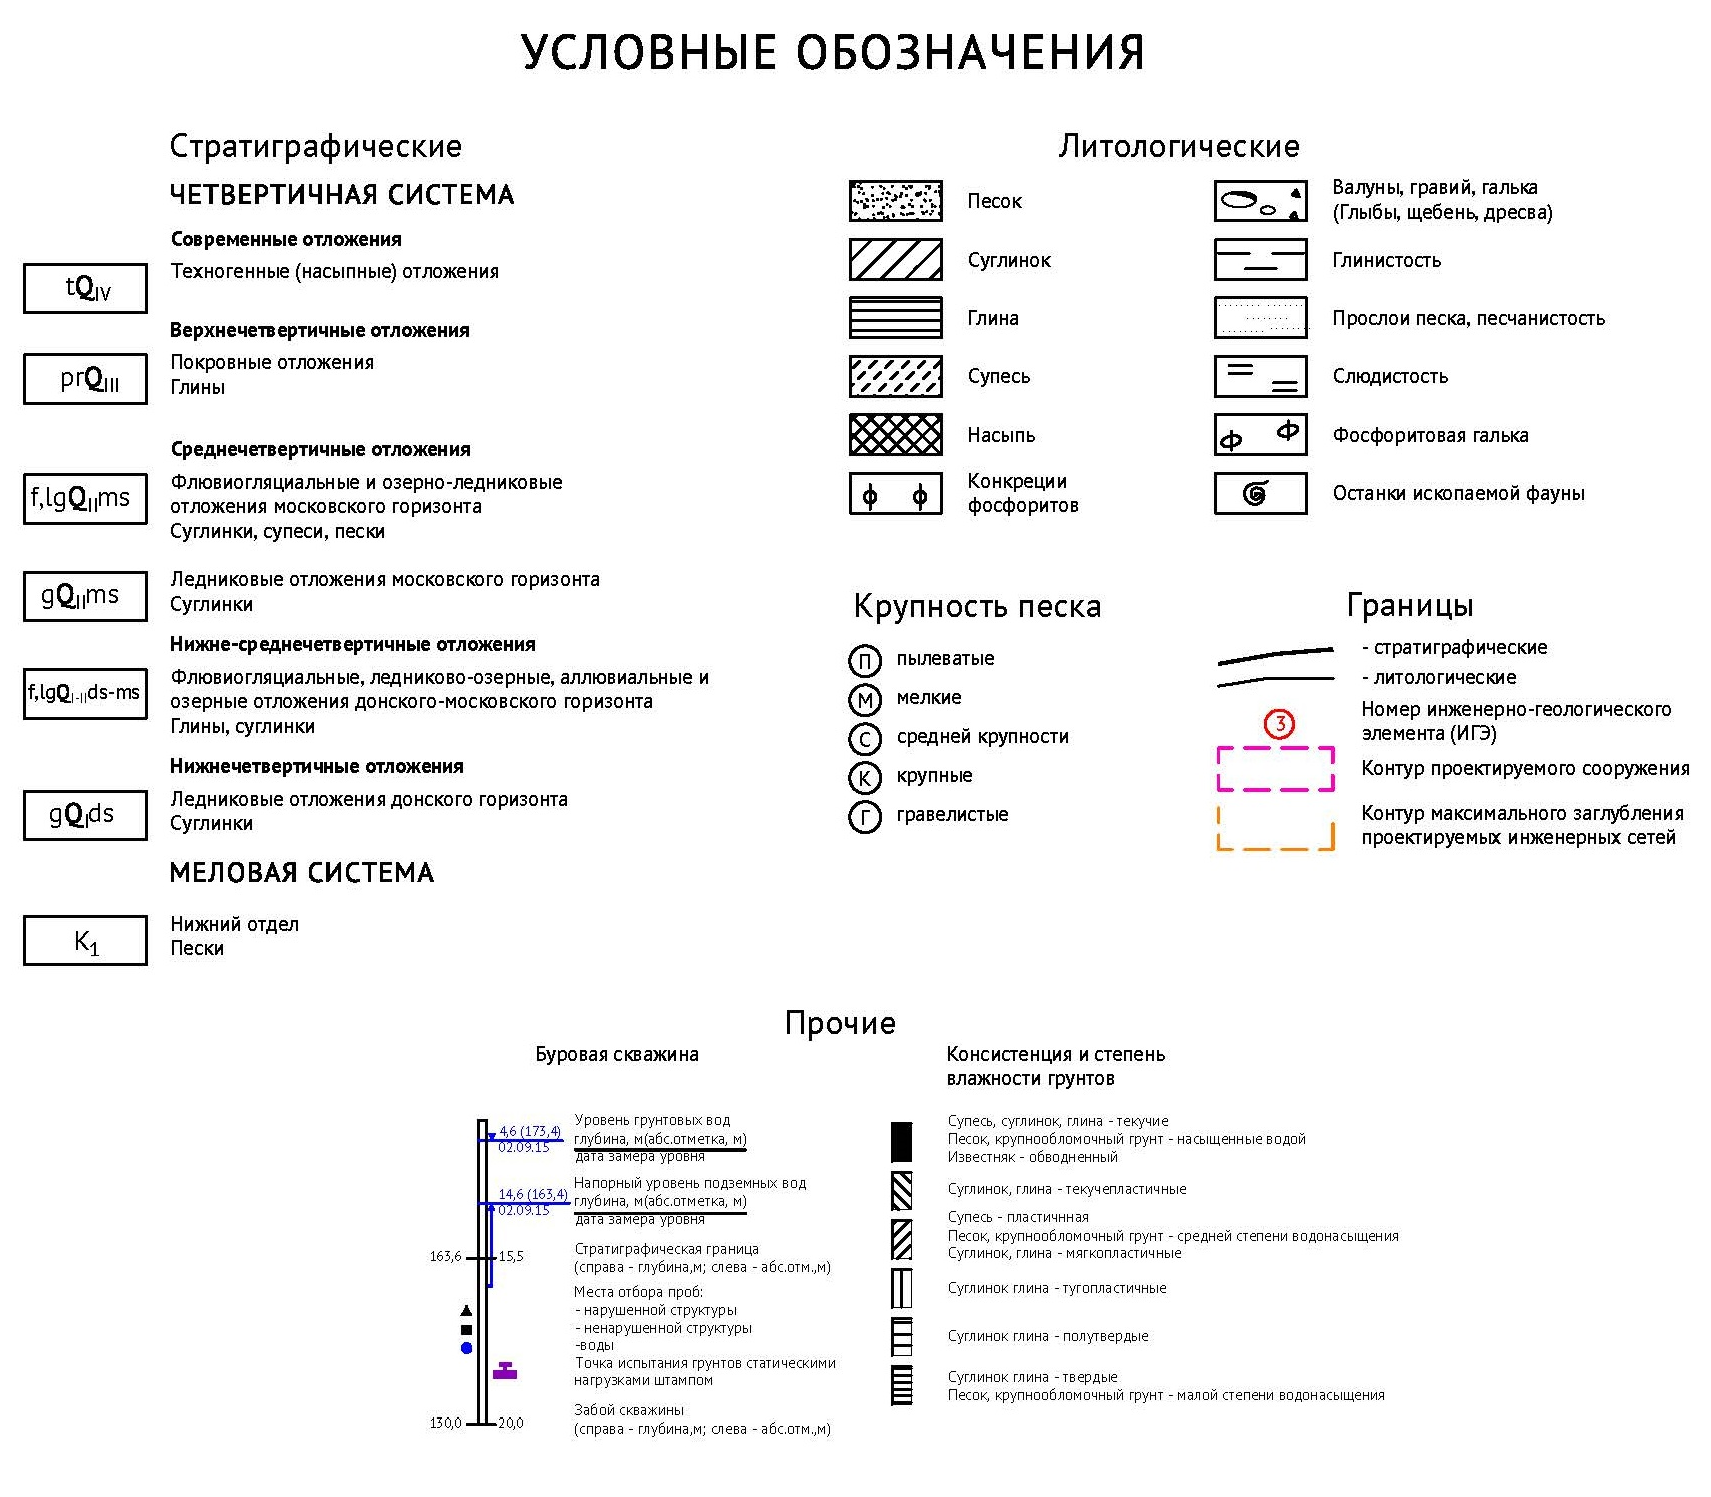
\includegraphics[scale=0.4]{images/usob.png}
  }
  \caption{Условные обозначения к инженерно-геологическому разрезу (Технический отчет. Саларьево-парк, 2019)}\label{fig:fig}
\end{figure}

 %\input{images/razrez.jpg}   
%\begin{sidewaysfigure}[ht]
%  \centerfloat{
%    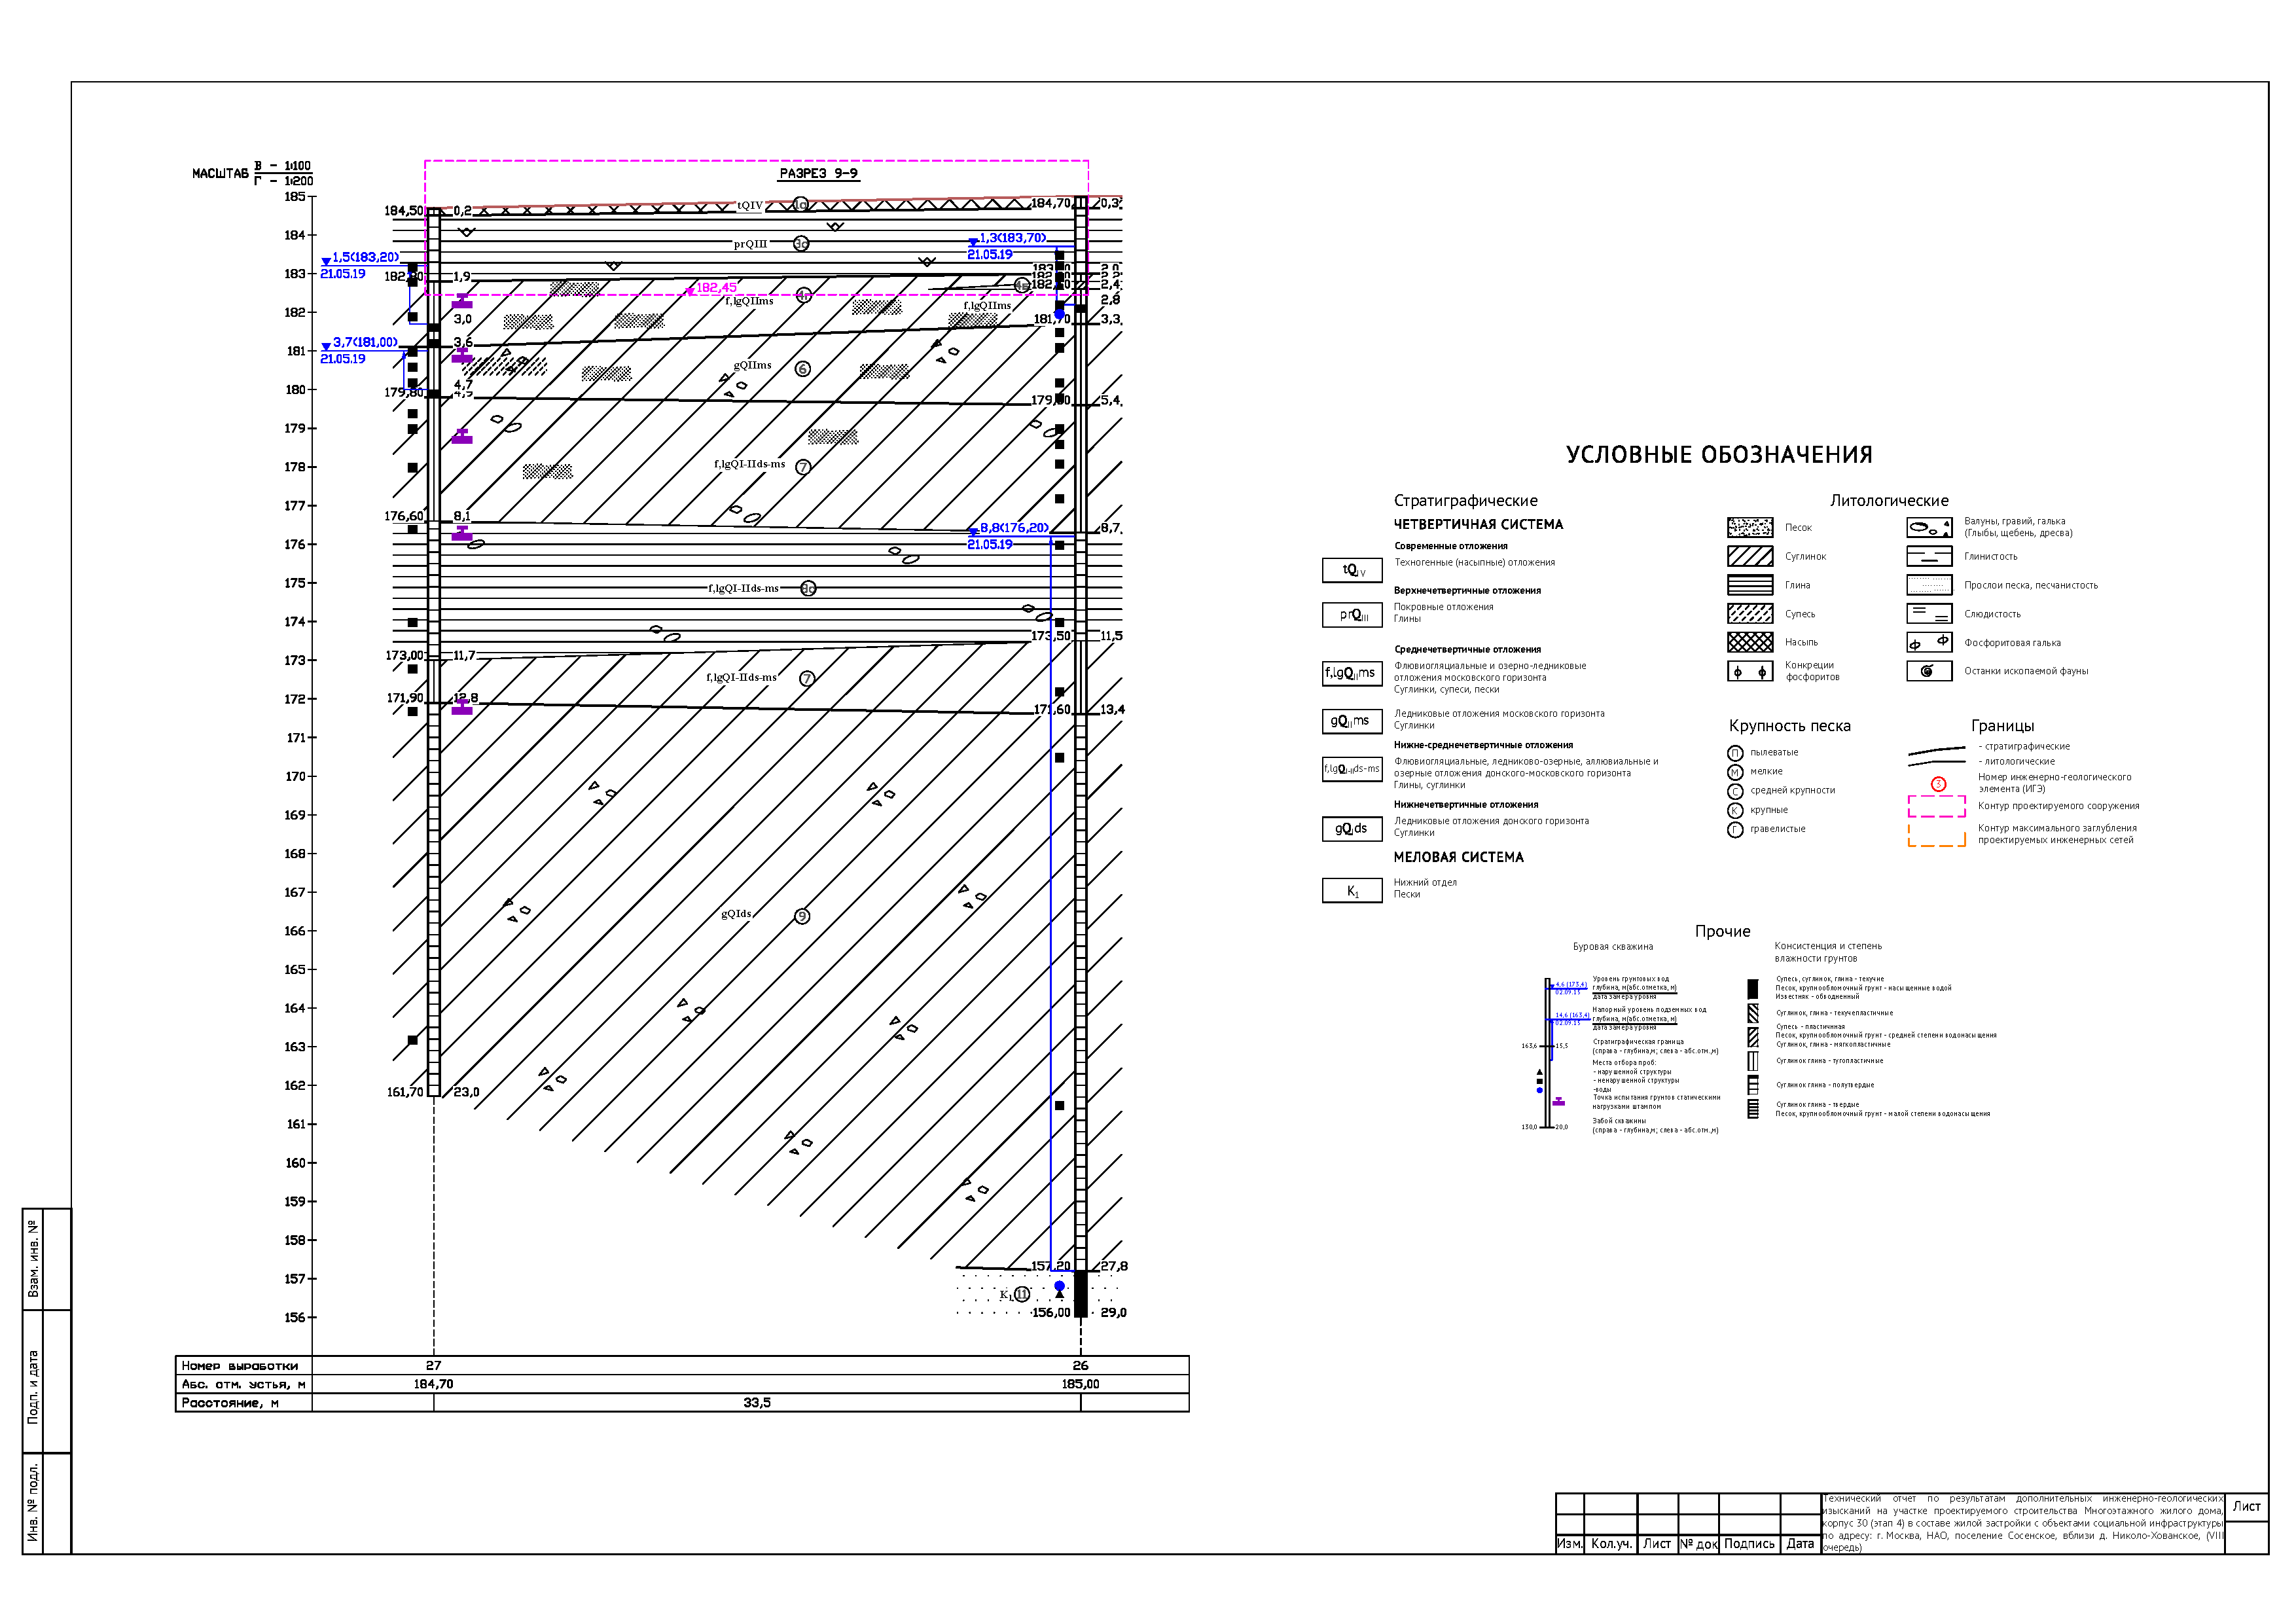
\includepdf[pages=-]{images/9-9.pdf}
%    \caption{Инженерно-геологический разрез}}
%\end{sidewaysfigure}


\begin{landscape}
\chapter{Физические свойства грунтов}\label{app:phisics}

%\begin{sidewaystable}[p]
   % \centering
   % \tiny
   % \caption{Физические свойства грунтов}
   % \begin{tabular}{@{}|l|r|r|r|r|r|r|r|r|r|r|p{4.8cm}|c|@{}}
   % \hline
   % Номер  & Глубина, \si{\meter} & $W$, д. е. & $W_l$, д. е. & $W_p$, д. е. & $I_p$ д .е & $I_l$, д.е. & $\rho$, г/\si{\centi\meter^3} & $\rho_s$, г/\si{\centi\meter^3} & $e$, д. е. & $S_r$, д. е. & Наименование   грунта                       & ИГЭ \\ \hline
   % GJ6805          & 3,5        & 0,171                        & 0,238   & 0,134  & 0,105  & 0,36     & 2,17     & 2,72      & 0,471   & 0,99     & суглинок легкий\linebreak   песчанистый тугопластичный & 6   \\ \hline
   % GJ6807          & 4,8        & 0,156                        & 0,228   & 0,129  & 0,099  & 0,27     & 2,17     & 2,69      & 0,449   & 0,95     & суглинок легкий\linebreak   песчанистый тугопластичный & 6   \\ \hline
   % GJ6838          & 4,3        & 0,150                        & 0,200   & 0,110  & 0,090  & 0,41     & 2,18     & 2,68      & 0,415   & 0,96     & суглинок легкий\linebreak  песчанистый тугопластичный & 6   \\\hline
   % GJ6835          & 3,5        & 0,150                        & 0,200   & 0,110  & 0,090  & 0,36     & 2,17     & 2,72      & 0,433   & 0,91     & суглинок легкий\linebreak   песчанистый тугопластичный & 6   \\ \hline
   % GJ6809          & 6,0        & 0,269                        & 0,322   & 0,210  & 0,112  & 0,53     & 1,97     & 2,72      & 0,752   & 0,97     & суглинок   мягкопластичный                   & 7   \\ \hline
   % GJ6810          & 6,4        & 0,251                        & 0,342   & 0,231  & 0,111  & 0,18     & 1,99     & 2,72      & 0,714   & 0,96     & суглинок полутвердый                         & 7   \\ \hline
   % GJ6821          & 6,7        & 0,233                        & 0,309   & 0,191  & 0,118  & 0,35     & 2,01     & 2,72      & 0,668   & 0,95     & суглинок   тугопластичный                    & 7   \\ \hline
   % GJ6898          & 12,1       & 0,240                        & 0,320   & 0,180  & 0,140  & 0,44     & 2,04     & 2,72      & 0,655   & 0,99     & суглинок тяжелый\linebreak   пылеватый тугопластичный  & 7   \\ \hline
   % GJ6874          & 7,4        & 0,240                        & 0,340   & 0,180  & 0,160  & 0,34     & 2,01     & 2,72      & 0,675   & 0,96     & суглинок тяжелый\linebreak   пылеватый тугопластичный  & 7   \\ \hline
   % GJ6888          & 10,2       & 0,230                        & 0,440   & 0,190  & 0,250  & 0,18     & 2,03     & 2,72      & 0,658   & 0,97     & глина легкая\linebreak   пылеватая полутвердая         & 8   \\ \hline
   % GJ6890          & 10,6       & 0,220                        & 0,410   & 0,170  & 0,230  & 0,18     & 2,07     & 2,72      & 0,602   & 0,98     & глина легкая\linebreak   песчанистая полутвердая       & 8   \\ \hline
   % GJ6852          & 10,3       & 0,210                        & 0,400   & 0,170  & 0,220  & 0,15     & 2,09     & 2,74      & 0,580   & 0,97     & глина полутвердая                            & 8   \\ \hline
   % GJ6889          & 10,4       & 0,220                        & 0,410   & 0,170  & 0,240  & 0,18     & 2,06     & 2,74      & 0,620   & 0,96     & глина полутвердая                            & 8   \\ \hline
   % GJ6822          & 8,3        & 0,244                        & 0,441   & 0,223  & 0,218  & 0,09     & 2,01     & 2,68      & 0,695   & 0,96     & глина полутвердая                            & 8   \\ \hline
   % GJ6884          & 9,2        & 0,220                        & 0,400   & 0,200  & 0,200  & 0,14     & 2,03     & 2,72      & 0,644   & 0,95     & глина легкая\linebreak   пылеватая полутвердая         & 8   \\ \hline
   % GJ6846          & 8,3        & 0,210                        & 0,510   & 0,210  & 0,310  & 0,02     & 2,08     & 2,72      & 0,585   & 0,99     & глина тяжелая\linebreak   полутвердая                  & 8   \\ \hline
   % GJ6855          & 11,7       & 0,192                        & 0,364   & 0,163  & 0,202  & 0,14     & 2,08     & 2,67      & 0,573   & 0,92     & глина легкая\linebreak   песчанистая полутвердая       & 9   \\ \hline
   % GJ6859          & 12,5       & 0,187                        & 0,374   & 0,166  & 0,208  & 0,1      & 2,10     & 2,72      & 0,549   & 0,93     & глина полутвердая                            & 9   \\ \hline
   % GJ6865          & 14,7       & 0,156                        & 0,312   & 0,134  & 0,179  & 0,12     & 2,18     & 2,72      & 0,442   & 0,94     & глина легкая\linebreak   песчанистая полутвердая       & 9   \\ \hline
   % GJ68A3          & 13,5       & 0,180                        & 0,330   & 0,150  & 0,180  & 0,18     & 2,10     & 2,68      & 0,509   & 0,95     & глина легкая\linebreak   песчанистая полутвердая       & 9   \\ \hline
   % GJ68B7          & 16,9       & 0,120                        & 0,300   & 0,130  & 0,170  & -0,06    & 2,26     & 2,72      & 0,354   & 0,94     & глина легкая       & 9   \\ \hline
   % GJ68A7          & 14,6       & 0,130                        & 0,290   & 0,140  & 0,160  & 0,08     & 2,23     & 2,72      & 0,372   & 0,91     & глина легкая                              & 9   \\ \hline
   % GJ6856          & 11,9       & 0,210                        & 0,380   & 0,160  & 0,210  & 0,22     & 2,09     & 2,74      & 0,588   & 0,97     & глина полутвердая                            & 9   \\ \hline
   % GJ68A0          & 12,6       & 0,180                        & 0,320   & 0,140  & 0,180  & 0,00     & 2,13     & 2,71      & 0,499   & 0,98     & глина легкая\linebreak   песчанистая полутвердая       & 9   \\ \hline
   % GJ6864          & 14,3       & 0,150                        & 0,310   & 0,140  & 0,170  & 0,06     & 2,19     & 2,72      & 0,433   & 0,97     & глина легкая \linebreak  песчанистая полутвердая       & 9   \\ \hline
   % \bottomrule 
   % \end{tabular}
   % \end{sidewaystable}

    \begin{table}[h]
      \small
      \centering
      \tiny
      \caption{Физические свойства грунтов}
      \begin{tabular}{@{}|l|r|r|r|r|r|r|r|r|r|r|r|@{}}
      \hline
      Номер  & Глубина, \si{\meter} & $W$, д. е. & $W_l$, д. е. & $W_p$, д. е. & $I_p$ д .е & $I_l$, д.е. & $\rho$, г/\si{\centi\meter^3} & $\rho_s$, г/\si{\centi\meter^3} & $e$, д. е. & $S_r$, д. е. & Наименование   грунта, ИГЭ \\ \hline
      GJ6805          & 3,5        & 0,171                        & 0,238   & 0,134  & 0,105  & 0,36     & 2,17     & 2,72      & 0,471   & 0,99     & суглинок легкий  тугопластичный, 6   \\ \hline
      GJ6807          & 4,8        & 0,156                        & 0,228   & 0,129  & 0,099  & 0,27     & 2,17     & 2,69      & 0,449   & 0,95     & суглинок легкий   тугопластичный, 6   \\ \hline
      GJ6838          & 4,3        & 0,150                        & 0,200   & 0,110  & 0,090  & 0,41     & 2,18     & 2,68      & 0,415   & 0,96     & суглинок легкий   тугопластичный, 6   \\\hline
      GJ6835          & 3,5        & 0,150                        & 0,200   & 0,110  & 0,090  & 0,36     & 2,17     & 2,72      & 0,433   & 0,91     & суглинок легкий   тугопластичный, 6   \\ \hline
      GJ6809          & 6,0        & 0,269                        & 0,322   & 0,210  & 0,112  & 0,53     & 1,97     & 2,72      & 0,752   & 0,97     & суглинок   мягкопластичный, 7   \\ \hline
      GJ6810          & 6,4        & 0,251                        & 0,342   & 0,231  & 0,111  & 0,18     & 1,99     & 2,72      & 0,714   & 0,96     & суглинок    полутвердый, 7   \\ \hline
      GJ6821          & 6,7        & 0,233                        & 0,309   & 0,191  & 0,118  & 0,35     & 2,01     & 2,72      & 0,668   & 0,95     & суглинок   тугопластичный, 7   \\ \hline
      GJ6898          & 12,1       & 0,240                        & 0,320   & 0,180  & 0,140  & 0,44     & 2,04     & 2,72      & 0,655   & 0,99     & суглинок тяжелый   тугопластичный, 7   \\ \hline
      GJ6874          & 7,4        & 0,240                        & 0,340   & 0,180  & 0,160  & 0,34     & 2,01     & 2,72      & 0,675   & 0,96     & суглинок тяжелый   тугопластичный, 7   \\ \hline
      GJ6888          & 10,2       & 0,230                        & 0,440   & 0,190  & 0,250  & 0,18     & 2,03     & 2,72      & 0,658   & 0,97     & глина легкая    полутвердая, 8   \\ \hline
      GJ6890          & 10,6       & 0,220                        & 0,410   & 0,170  & 0,230  & 0,18     & 2,07     & 2,72      & 0,602   & 0,98     & глина легкая    полутвердая, 8   \\ \hline
      GJ6852          & 10,3       & 0,210                        & 0,400   & 0,170  & 0,220  & 0,15     & 2,09     & 2,74      & 0,580   & 0,97     & глина полутвердая, 8   \\ \hline
      GJ6889          & 10,4       & 0,220                        & 0,410   & 0,170  & 0,240  & 0,18     & 2,06     & 2,74      & 0,620   & 0,96     & глина полутвердая, 8   \\ \hline
      GJ6822          & 8,3        & 0,244                        & 0,441   & 0,223  & 0,218  & 0,09     & 2,01     & 2,68      & 0,695   & 0,96     & глина полутвердая, 8   \\ \hline
      GJ6884          & 9,2        & 0,220                        & 0,400   & 0,200  & 0,200  & 0,14     & 2,03     & 2,72      & 0,644   & 0,95     & глина легкая    полутвердая, 8   \\ \hline
      GJ6846          & 8,3        & 0,210                        & 0,510   & 0,210  & 0,310  & 0,02     & 2,08     & 2,72      & 0,585   & 0,99     & глина тяжелая   полутвердая, 8   \\ \hline
      GJ6855          & 11,7       & 0,192                        & 0,364   & 0,163  & 0,202  & 0,14     & 2,08     & 2,67      & 0,573   & 0,92     & глина легкая    полутвердая, 9   \\ \hline
      GJ6859          & 12,5       & 0,187                        & 0,374   & 0,166  & 0,208  & 0,1      & 2,10     & 2,72      & 0,549   & 0,93     & глина полутвердая, 9   \\ \hline
      GJ6865          & 14,7       & 0,156                        & 0,312   & 0,134  & 0,179  & 0,12     & 2,18     & 2,72      & 0,442   & 0,94     & глина легкая    полутвердая, 9   \\ \hline
      GJ68A3          & 13,5       & 0,180                        & 0,330   & 0,150  & 0,180  & 0,18     & 2,10     & 2,68      & 0,509   & 0,95     & глина легкая    полутвердая, 9   \\ \hline
      GJ68B7          & 16,9       & 0,120                        & 0,300   & 0,130  & 0,170  & -0,06    & 2,26     & 2,72      & 0,354   & 0,94     & глина легкая, 9   \\ \hline
      GJ68A7          & 14,6       & 0,130                        & 0,290   & 0,140  & 0,160  & 0,08     & 2,23     & 2,72      & 0,372   & 0,91     & глина легкая, 9   \\ \hline
      GJ6856          & 11,9       & 0,210                        & 0,380   & 0,160  & 0,210  & 0,22     & 2,09     & 2,74      & 0,588   & 0,97     & глина полутвердая, 9   \\ \hline
      GJ68A0          & 12,6       & 0,180                        & 0,320   & 0,140  & 0,180  & 0,00     & 2,13     & 2,71      & 0,499   & 0,98     & глина легкая    полутвердая, 9   \\ \hline
      GJ6864          & 14,3       & 0,150                        & 0,310   & 0,140  & 0,170  & 0,06     & 2,19     & 2,72      & 0,433   & 0,97     & глина легкая    полутвердая, 9   \\ \hline
      \bottomrule 
      \end{tabular}
      \end{table}
    \end{landscape}

\chapter{Результаты рентгеноструктурного анализа}\label{app:difrac}
(инж. 1 кат. С.А. Гаранина, вед. инж. С.В. Закусин, ст.н.с. В.В. Крупская)

\begin{figure}[ht]
    \centerfloat{
      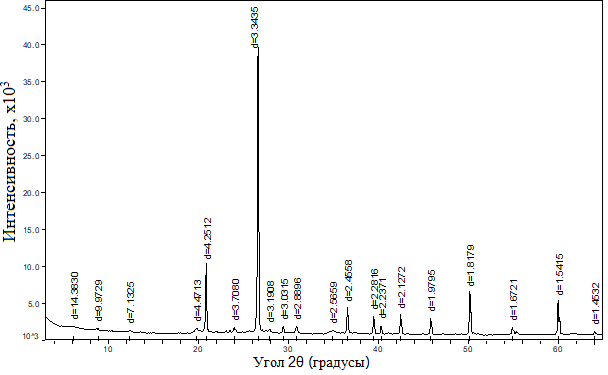
\includegraphics[scale=1.05]{dif68B7.png}
    }
    \caption{Рентгеновская дифракционная картина образца GJ68B7 (ИГЭ-9, суглинки полутвердые)}\label{fig:fig}
  \end{figure}

  \begin{figure}[ht]
    \centerfloat{
      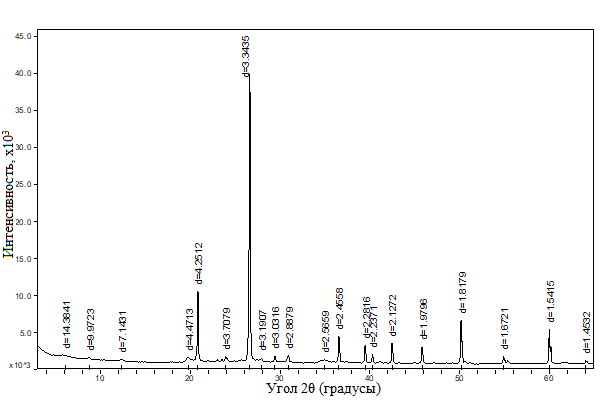
\includegraphics[scale=1.05]{dif68D4.png}
    }
    \caption{Рентгеновская дифракционная картина образца GJ68D4 (ИГЭ-9, суглинки полутвердые)}\label{fig:fig}
  \end{figure}

  \begin{figure}[ht]
    \centerfloat{
      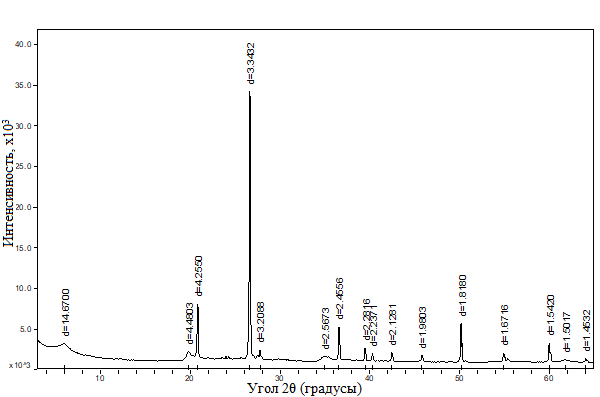
\includegraphics[scale=1.1]{dif6890.png}
    }
    \caption{Рентгеновская дифракционная картина образца GJ6890 (ИГЭ-8а, глины полутвердые)}\label{fig:fig}
  \end{figure}

  \begin{figure}[ht]
    \centerfloat{
      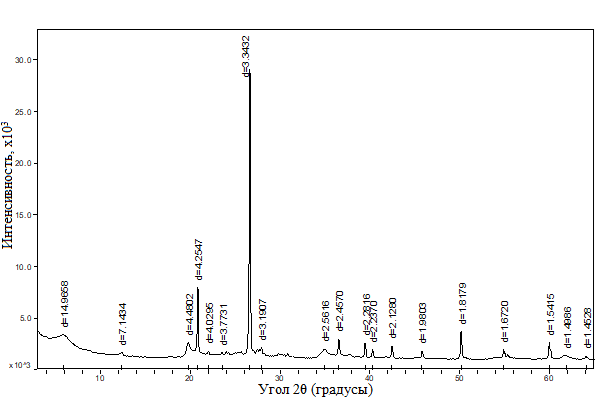
\includegraphics[scale=1.1]{dif6881.png}
    }
    \caption{Рентгеновская дифракционная картина образца GJ6881 (ИГЭ-8а, глины полутвердые)}\label{fig:fig}
  \end{figure}

  \begin{figure}[ht]
    \centerfloat{
      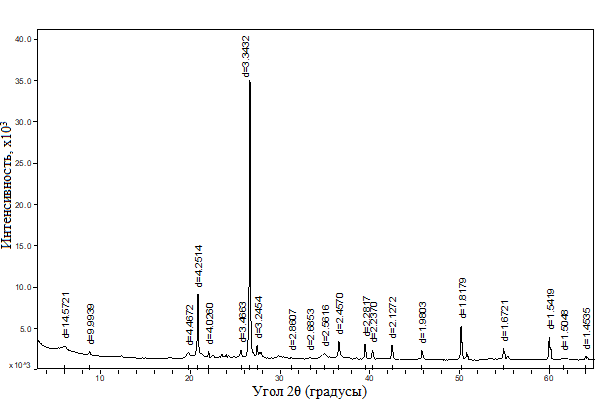
\includegraphics[scale=1.1]{dif6898.png}
    }
    \caption{Рентгеновская дифракционная картина образца GJ6898 (ИГЭ-7, суглинки тугопластичные)}\label{fig:fig}
  \end{figure}

  \begin{figure}[ht]
    \centerfloat{
      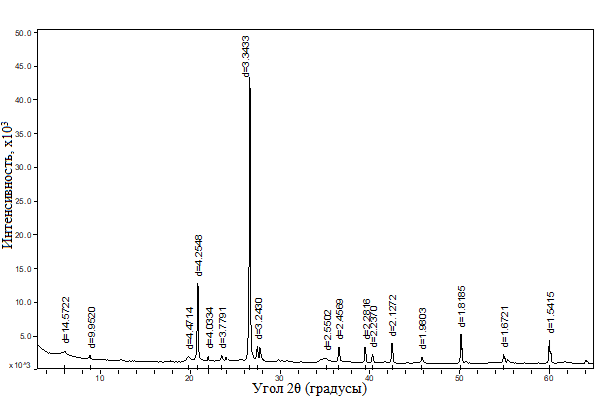
\includegraphics[scale=1.1]{dif6899.png}
    }
    \caption{Рентгеновская дифракционная картина образца GJ6899 (ИГЭ-7, суглинки тугопластичные)}\label{fig:fig}
  \end{figure}

\chapter{Компрессионные кривые}\label{app:oedometer}
\small
\pgfplotsset{
    % discard if not/.style 2 args={
    %     x filter/.code={
    %         \edef\tempa{\thisrow{#1}}
    %         \edef\tempb{#2}
    %         \ifx\tempa\tempb
    %         \else
    %             \def\pgfmathresult{inf}
    %         \fi
    %     }
    % }
}

\pgfplotsset{
% 	%samples=15,
	width= 0.9\linewidth,
	height = 10cm,
	xlabel={Вертикальное эфф. напряжение $\\sigma_1$, кПа},
	ylabel={Отн. верт. деформация $\epsilon_1$, д. е.},
% 	%extra y ticks={45},
	legend pos=north west,
	y dir=reverse, 
	y tick label style={
		/pgf/number format/.cd,
			fixed,
			fixed zerofill,
			precision=3,
		/tikz/.cd
	},
	ylabel near ticks,
	% ylabel shift = 5cm,
% 	% clip mode=individual,
	x tick label style={
        /pgf/number format/set thousands separator={\,},
		/pgf/number format/.cd,
			fixed,
			fixed zerofill
        /tikz/.cd
	},
    xticklabel={
        \pgfkeys{ /pgf/number format/fixed, 
            /pgf/number format/fixed zerofill, 
            /pgf/number format/precision=0} 
        \pgfmathparse{exp(\tick)}
        \pgfmathprintnumber{\pgfmathresult}
    }
}

{
\tiny

\begin{figure}[ht]
	\begin{tikzpicture}
		% \centering
		\begin{semilogxaxis}
		\addplot[mark=*, red] table [x=Sigma, y=Epsilon, col sep=semicolon] {data/GJ6805.csv};
		\end{semilogxaxis}
	\end{tikzpicture}
	\caption{Компрессионная кривая образца \texttt{GJ6805}}
\end{figure}

\begin{figure}
\begin{tikzpicture}
	\begin{semilogxaxis}[y dir=reverse]
	\addplot[mark=*, red] table [x=Sigma, y=Epsilon, col sep=semicolon] {data/GJ6807.csv};
	\end{semilogxaxis}
\end{tikzpicture}
\caption{\texttt{GJ6807}}
\end{figure}

\begin{figure}
\begin{tikzpicture}
	\begin{semilogxaxis}[y dir=reverse]
	\addplot[mark=*, red] table [x=Sigma, y=Epsilon, col sep=semicolon] {data/GJ6838.csv};
	\end{semilogxaxis}
\end{tikzpicture}
\caption{Компрессионная кривая образца \texttt{GJ6838}}
\end{figure}

\begin{figure}
\begin{tikzpicture}
	\begin{semilogxaxis}[y dir=reverse]
	\addplot[mark=*, red] table [x=Sigma, y=Epsilon, col sep=semicolon] {data/GJ6809.csv};
	\end{semilogxaxis}
\end{tikzpicture}
\caption{Компрессионная кривая образца \texttt{GJ6809}}
\end{figure}

\begin{figure}

\begin{tikzpicture}
	\begin{semilogxaxis}[y dir=reverse]
	\addplot[mark=*, red] table [x=Sigma, y=Epsilon, col sep=semicolon] {data/GJ6810.csv};
	\end{semilogxaxis}
\end{tikzpicture}
\caption{Компрессионная кривая образца \texttt{GJ6810}}
\end{figure}

\begin{figure}
\begin{tikzpicture}
	\begin{semilogxaxis}[y dir=reverse]
	\addplot[mark=*, red] table [x=Sigma, y=Epsilon, col sep=semicolon] {data/GJ6821.csv};
	\end{semilogxaxis}
\end{tikzpicture}
\caption{Компрессионная кривая образца \texttt{GJ6821}}
\end{figure}

\begin{figure}
\begin{tikzpicture}
	\begin{semilogxaxis}[y dir=reverse]
	\addplot[mark=*, red] table [x=Sigma, y=Epsilon, col sep=semicolon] {data/GJ6898.csv};
	\end{semilogxaxis}
\end{tikzpicture}
\caption{\texttt{GJ6898}}
\end{figure}

\begin{figure}
\begin{tikzpicture}
	\begin{semilogxaxis}[y dir=reverse]
	\addplot[mark=*, red] table [x=Sigma, y=Epsilon, col sep=semicolon] {data/GJ6822.csv};
	\end{semilogxaxis}
\end{tikzpicture}
\caption{Компрессионная кривая образца \texttt{GJ6822}}
\end{figure}

\begin{figure}
\begin{tikzpicture}
	\begin{semilogxaxis}[y dir=reverse]
	\addplot[mark=*, red] table [x=Sigma, y=Epsilon, col sep=semicolon] {data/GJ6884.csv};
	\end{semilogxaxis}
\end{tikzpicture}
\caption{Компрессионная кривая образца \texttt{GJ6884}}
\end{figure}

\begin{figure}
\begin{tikzpicture}
	\begin{semilogxaxis}[y dir=reverse]
	\addplot[mark=*, red] table [x=Sigma, y=Epsilon, col sep=semicolon] {data/GJ6846.csv};
	\end{semilogxaxis}§
\end{tikzpicture}
\caption{Компрессионная кривая образца \texttt{GJ6846}}
\end{figure}

\begin{figure}
\begin{tikzpicture}
	\begin{semilogxaxis}[y dir=reverse]
	\addplot[mark=*, red] table [x=Sigma, y=Epsilon, col sep=semicolon] {data/GJ6855.csv};
	\end{semilogxaxis}
\end{tikzpicture}
\caption{Компрессионная кривая образца \texttt{GJ6855}}
\end{figure}

\begin{figure}
\begin{tikzpicture}
	\begin{semilogxaxis}[y dir=reverse]
	\addplot[mark=*, red] table [x=Sigma, y=Epsilon, col sep=semicolon] {data/GJ6859.csv};
	\end{semilogxaxis}
\end{tikzpicture}
\caption{Компрессионная кривая образца \texttt{GJ6859}}
\end{figure}


\begin{figure}
\begin{tikzpicture}
	\begin{semilogxaxis}[y dir=reverse]
	\addplot[mark=*, red] table [x=Sigma, y=Epsilon, col sep=semicolon] {data/GJ6865.csv};
	\end{semilogxaxis}
\end{tikzpicture}
\caption{Компрессионная кривая образца \texttt{GJ6865}}
\end{figure}

	
\begin{figure}
\begin{tikzpicture}
	\begin{semilogxaxis}[y dir=reverse]
	\addplot[mark=*, red] table [x=Sigma, y=Epsilon, col sep=semicolon] {data/GJ68A3.csv};
	\end{semilogxaxis}
\end{tikzpicture}
\caption{Компрессионная кривая образца \texttt{GJ68A3}}
\end{figure}

	
\begin{figure}
\begin{tikzpicture}
	\begin{semilogxaxis}[y dir=reverse]
	\addplot[mark=*, red] table [x=Sigma, y=Epsilon, col sep=semicolon] {data/GJ68B7.csv};
	\end{semilogxaxis}
\end{tikzpicture}
\caption{Компрессионная кривая образца \texttt{GJ68B7}}
\end{figure}
}

\chapter{Построения для определения напряжения предуплотения}\label{app:method}
% Inkscape figure
\begin{figure}[h!]
    {\centering
      \def\svgwidth{11cm} % используем для изменения размера, если надо
      %\includesvg{figs/drawing}
      \small
      \subbottom[Метод Казагранде]{%
      \centering
      \input{images/oedometerCazagrande+monolith+1.pdf_tex} }
      \hfill 
      \\
      \hfill  
      \def\svgwidth{11cm}
      \subbottom[Метод Беккера]{%
      \centering
      \input{images/oedometerBecker+monolith+1.pdf_tex}}
      \hfill 
      }
      \caption{Определение напряжения предуплотнения образца \texttt{GJ6805} (ИГЭ-6, суглинки тугопластичные)}
      \label{img:6805}
    \end{figure}
    
    \begin{figure}
        {\centering
        \small
          %\def\svgwidth{5cm} % используем для изменения размера, если надо
          %\includesvg{figs/drawing}
          \subbottom[Метод Казагранде]{%
          \centering
          \input{images/oedometerCazagrande+monolith+2.pdf_tex} }
          \hfill 
          \\
          \hfill  
          \subbottom[Метод Беккера]{%
          \centering
          \input{images/oedometerBecker+monolith+2.pdf_tex}}
          \hfill 
          }
          \caption{Определение напряжения предуплотнения образца \texttt{GJ6807} (ИГЭ-6, суглинки тугопластичные)}
          \label{img:6807}
    \end{figure}
    
    \begin{figure}
        {\centering
        \small
            %\def\svgwidth{5cm} % используем для изменения размера, если надо
            %\includesvg{figs/drawing}
            \subbottom[Метод Казагранде]{%
            \centering
            \input{images/oedometerCazagrande+monolith+3.pdf_tex} }
            \hfill 
            \\
            \hfill  
            \subbottom[Метод Беккера]{%
            \centering
            \input{images/oedometerBecker+monolith+3.pdf_tex}}
            \hfill 
            }
            \caption{Определение напряжения предуплотнения образца \texttt{GJ6838} (ИГЭ-6, суглинки тугопластичные)}
            \label{img:6838}
    \end{figure}
    
    
    \begin{figure}
        {\centering
        \small
            %\def\svgwidth{5cm} % используем для изменения размера, если надо
            %\includesvg{figs/drawing}
            \subbottom[Метод Казагранде]{%
            \centering
            \input{images/oedometerCazagrande+monolith+4.pdf_tex} }
            \hfill 
            \\
            \hfill  
            \subbottom[Метод Беккера]{%
            \centering
            \input{images/oedometerBecker+monolith+4.pdf_tex}}
            \hfill 
            }
            \caption{Определение напряжения предуплотнения образца \texttt{GJ6809} (ИГЭ-7, суглинки тугопластичные)}
            \label{img:6809}
    \end{figure}
    
    \begin{figure}
        {\centering
        \small
            %\def\svgwidth{5cm} % используем для изменения размера, если надо
            %\includesvg{figs/drawing}
            \subbottom[Метод Казагранде]{%
            \centering
            \input{images/oedometerCazagrande+monolith+5.pdf_tex} }
            \hfill 
            \\
            \hfill  
            \subbottom[Метод Беккера]{%
            \centering
            \input{images/oedometerBecker+monolith+5.pdf_tex}}
            \hfill 
            }
            \caption{Определение напряжения предуплотнения образца \texttt{GJ6810} (ИГЭ-7, суглинки тугопластичные)}
            \label{img:6810}
    \end{figure}
    
    \begin{figure}
        {\centering
        \small
            %\def\svgwidth{5cm} % используем для изменения размера, если надо
            %\includesvg{figs/drawing}
            \subbottom[Метод Казагранде]{%
            \centering
            \input{images/oedometerCazagrande+monolith+6.pdf_tex} }
            \hfill 
            \\
            \hfill  
            \subbottom[Метод Беккера]{%
            \centering
            \input{images/oedometerBecker+monolith+6.pdf_tex}}
            \hfill 
            }
            \caption{Определение напряжения предуплотнения образца \texttt{GJ6821} (ИГЭ-7, суглинки тугопластичные)}
            \label{img:6821}
    \end{figure}
    
    \begin{figure}
        {\centering
        \small
            %\def\svgwidth{5cm} % используем для изменения размера, если надо
            %\includesvg{figs/drawing}
            \subbottom[Метод Казагранде]{%
            \centering
            \input{images/oedometerCazagrande+monolith+7.pdf_tex} }
            \hfill 
            \\
            \hfill  
            \subbottom[Метод Беккера]{%
            \centering
            \input{images/oedometerBecker+monolith+7.pdf_tex}}
            \hfill 
            }
            \caption{Определение напряжения предуплотнения образца \texttt{GJ6898} (ИГЭ-7, суглинки тугопластичные)}
            \label{img:6898}
    \end{figure}
    
    \begin{figure}
        {\centering
        \small
            %\def\svgwidth{5cm} % используем для изменения размера, если надо
            %\includesvg{figs/drawing}
            \subbottom[Метод Казагранде]{%
            \centering
            \input{images/oedometerCazagrande+monolith+8.pdf_tex} }
            \hfill 
            \\
            \hfill  
            \subbottom[Метод Беккера]{%
            \centering
            \input{images/oedometerBecker+monolith+8.pdf_tex}}
            \hfill 
            }
            \caption{Определение напряжения предуплотнения образца \texttt{GJ6822} (ИГЭ-8а, глины полутвердые)}
            \label{img:6822}
    \end{figure}
    
    \begin{figure}
        {\centering
        \small
            %\def\svgwidth{5cm} % используем для изменения размера, если надо
            %\includesvg{figs/drawing}
            \subbottom[Метод Казагранде]{%
            \centering
            \input{images/oedometerCazagrande+monolith+9.pdf_tex} }
            \hfill 
            \\
            \hfill  
            \subbottom[Метод Беккера]{%
            \centering
            \input{images/oedometerBecker+monolith+9.pdf_tex}}
            \hfill 
        }
        \caption{Определение напряжения предуплотнения образца \texttt{GJ6884} (ИГЭ-8а, глины полутвердые)}
        \label{img:6884}
    \end{figure}
    
    \begin{figure}
        {\centering
        \small
            %\def\svgwidth{5cm} % используем для изменения размера, если надо
            %\includesvg{figs/drawing}
            \subbottom[Метод Казагранде]{%
            \centering
            \input{images/oedometerCazagrande+monolith+10.pdf_tex} }
            \hfill 
            \\
            \hfill  
            \subbottom[Метод Беккера]{%
            \centering
            \input{images/oedometerBecker+monolith+10.pdf_tex}}
            \hfill  
            }
            \caption{Определение напряжения предуплотнения образца \texttt{GJ6846} (ИГЭ-8а, глины полутвердые)}
            \label{img:6846}
    \end{figure}
    
    \begin{figure}
        {\centering
            %\def\svgwidth{5cm} % используем для изменения размера, если надо
            %\includesvg{figs/drawing}
            \small
            \subbottom[Метод Казагранде]{%
            \centering
            \input{images/oedometerCazagrande+monolith+11.pdf_tex} }
            \hfill 
            \\
            \hfill  
            \subbottom[Метод Беккера]{%
            \centering
            \input{images/oedometerBecker+monolith+11.pdf_tex}}
            \hfill  
            }
            \caption{Определение напряжения предуплотнения образца \texttt{GJ6855} (ИГЭ-9, суглинки полутвердые)}
            \label{img:6855}
    \end{figure}
    
    \begin{figure}
        {\centering
            %\def\svgwidth{5cm} % используем для изменения размера, если надо
            %\includesvg{figs/drawing}
            \small
            %\hfill
            \subbottom[Метод Казагранде]{%
            \centering
            \input{images/oedometerCazagrande+monolith+12.pdf_tex} }
            \hfill 
            \\
            \hfill   
            \subbottom[Метод Беккера]{%
            \centering
            \input{images/oedometerBecker+monolith+12.pdf_tex}}
            \hfill 
            }
            \caption{Определение напряжения предуплотнения образца \texttt{GJ6859} (ИГЭ-9, суглинки полутвердые)}
            \label{img:6859}
    \end{figure}
        
    \begin{figure}
        {\centering
            %\def\svgwidth{5cm} % используем для изменения размера, если надо
            %\includesvg{figs/drawing}
            \small
            %\hfill
            \subbottom[Метод Казагранде]{%
            \centering
            \input{images/oedometerCazagrande+monolith+13.pdf_tex} }
            \hfill 
            \\
            \hfill   
            \subbottom[Метод Беккера]{%
            \centering
            \input{images/oedometerBecker+monolith+13.pdf_tex}}
            \hfill 
            }
            \caption{Определение напряжения предуплотнения образца \texttt{GJ6865} (ИГЭ-9, суглинки полутвердые)}
            \label{img:6865}
    \end{figure}
        
    \begin{figure}
        {\centering
            %\def\svgwidth{5cm} % используем для изменения размера, если надо
            %\includesvg{figs/drawing}
            \small
            %\hfill
            \subbottom[Метод Казагранде]{%
            \centering
            \input{images/oedometerCazagrande+monolith+14.pdf_tex} }
            \hfill 
            \\
            \hfill   
            \subbottom[Метод Беккера]{%
            \centering
            \input{images/oedometerBecker+monolith+14.pdf_tex}}
            \hfill 
            }
            \caption{Определение напряжения предуплотнения образца \texttt{GJ68A3} (ИГЭ-9, суглинки полутвердые)}
            \label{img:68A3}
    \end{figure}
        
    \begin{figure}
        {\centering
            %\def\svgwidth{5cm} % используем для изменения размера, если надо
            %\includesvg{figs/drawing}
            \small
            %\hfill
            \subbottom[Метод Казагранде]{%
            \centering
            \input{images/oedometerCazagrande+monolith+15.pdf_tex} }
            \hfill 
            \\
            \hfill   
            \subbottom[Метод Беккера]{%
            \centering
            \input{images/oedometerBecker+monolith+15.pdf_tex}}
            \hfill 
            }
            \caption{Определение напряжения предуплотнения образца \texttt{GJ68B7} (ИГЭ-9, суглинки полутвердые)}
            \label{img:68B7}
    \end{figure}